\chapter{Обсуждение} \label{discussion}

\section{Изменения на молекулярном уровне у полевочьих, перешедших к подземному образу жизни}

В нашей работе получены данные по изменению уровня отбора в митохондриальных генах подземных грызунов, а также обнаружены характерные для них параллельные замены в ядерных генах. Помимо этого, мы сравнивали базовые характеристики митохондриальных геномов: GC-состав, его смещение, количество и порядок генов. 

\subsection{Изменение нуклеотиного состава митохондриальных геномов}

Оценка GC-состава показывает повышение количества этих нуклеотидов у подземных грызунов. Уровень смещения (GC-skew) у подземных грызунов сильнее, чем у наземных грызунов. Оно может быть связано с изменением количества нуклеотидов GC-пары. Несмотря на то, что разница в обоих случаях недостоверна, это может указывать на адаптивные следы в митохондриальном геноме. 

Смещение в сторону повышенного содержания A/T наблюдается в мтДНК многих видов (\cite{Ballard2004}). Это может быть вызвано факторами, влияющими на скорость повреждения ДНК (\cite{Martin1995}) и относительную доступность каждого нуклеотида в клеточной среде митохондрии (\cite{Xia1996}). AT-богатые геномы могут реплицироваться быстрее, чем GC-богатые и, при прочих равных, обладают избирательным преимуществом в гетероплазматической популяции (\cite{Ballard2000}). Поскольку у подземных грызунов снижен общий метаболический уровень, может также снижаться и скорость репликации митогеномов. Это, в том числе, и может повлечь обогащение GC-нуклеотидами и, помимо этого, обеспечить большую устойчивость перед активными формами кислорода. Зависимость между обогащением GC-нуклеотидов и увеличением значения GC-skew показана в работе (\cite{Saccone2000}), и вполне ожидаемо было обнаружить разницу в этом значении между подземными и наземными видами. 

Генный состав митохондрий среди всех изученных видов остается стабильным и неизменным. Переход к подземному образу жизни не повлек за собой изменение в порядке генов или удвоение каких-то конкретных блоков. 

\subsection{Ослабление уровня отбора}

Исторически, изучение адаптивности митохондриальных генов началось с гена \textit{CYTB}. Начатые с трудов Эндрюс (\cite{Andrews1998}), и в последующем повторенные целым рядом исследователей (\cite{Tomasco2014}; \cite{DaSilva2009}; \cite{DiRocco2006}; \cite{Shao2015}), работы свидетельствовали о наличии признаков положительного отбора при эволюции гена \textit{CYTB}. Дальнейшие исследования показали, что, несмотря на сильные функциональные ограничения, митохондриальная ДНК в целом может подвергаться положительному направленному отбору, например, в случаях, когда требуется энергоемкий образ жизни и/или есть ограничения в доступности кислорода (\cite{Tomasco2011}; \cite{Shen2010}; \cite{Blier2001}).

Нево (\cite{Nevo1999}) связывал изменения в гене \textit{CYTB} с экологическими различиями между хромосомными расами слепышей \textit{Spalax ehrenbergi}. Da Silva с коллегами (\cite{DaSilva2009}) обнаружили достоверную разницу в соотношении \textit{dN}/\textit{dS} ($\omega$) в независимых линиях подземных грызунов по сравнению с их наземными сестринскими видами. Это предполагает связь между эволюцией гена \textit{CYTB} и освоением гипоксической среды. Позднее это наблюдение было подтверждено для всех митохондриальных белок-кодирующих генов \textit{Octodontidae} (\cite{Tomasco2011}).

В нашем исследовании гена \textit{CYTB} мы также обнаружили ослабление отбора у некоторых подземных грызунов. Применяя стандартные подходы, мы показали, что (1) несколько филогенетически далеких подземных видов имеют одинаковые аминокислотные замены в цитохроме b, и эти замены, вероятно, важны для структуры белкового комплекса, (2) в последовательности гена \textit{CYTB} повышено соотношение между несинонимичными и синонимичными заменами ($\omega$) у подземных грызунов по сравнению с наземными и (3) восемь белковых доменов обладают повышенной частотой замен у подземных видов, тоже наблюдается в нескольких нуклеотидных позициях. Эти результаты согласуются с гипотезой о том, что колонизация подземной ниши способствует положительному отбору в генах мтДНК.

Признаки усиления положительного отбора были выявлены как при сравнении четырех видов \textit{Ellobius} с \textit{Arvicola}, \textit{Eothenomys} и \textit{Chionomys}, так и у \textit{L. mandarinus} при сравнении с другими видами \textit{Lasiopodomys} и \textit{Neodon}. Мы обнаружили достоверную разницу в значениях $\omega$, сравнивая \textit{T. subterraneus} с другими видами \textit{Terricola} и \textit{Microtus}, но в этом случае соотношение \textit{dN}/\textit{dS}, наоборот, было меньше для \textit{T. subterraneus}. Данные анализа RELAX согласуются с результатами codeml и показывают, что ген \textit{CYTB} у подземных грызунов подвержен ослаблению уровня отбора.


Результаты, полученные нами при исследовании всех белок-кодирующих митохондриальных генов, также говорят о вовлеченности митохондриального генома в адаптивный процесс. Метод оценки отбора по отдельным ветвям (branch model), который считается более точным и чувствительным, показал повышение уровня отбора в белок-кодирующих генах у подземных грызунов. Однако, мы наблюдаем различие в количестве генов с достоверным отличием у разных видов. Больше всего различий обнаружено у представителей рода \textit{Ellobius}: разница в отборе наблюдается во всех митохондриальных генах, кроме \textit{ND2,3,5,6} и \textit{COX3}. Два гена под отбором обнаружено у \textit{L. mandarinus}: \textit{COX3} и \textit{CYTB} и только один ген у \textit{Prometheomys} -- \textit{COX3}. У оставшихся представителей подземных грызунов не было обнаружено генов с достоверным отличием. Анализ RELAX подтвердил ослабление уровня отбора в митохондриальных генах у разных видов. Так, у представителей рода \textit{Ellobius} ослабление отбора наблюдается в 8 генах, у \textit{Prometheomys} --- в пяти (при сравнении с первой радиацией) и одном при сравнении с хомяками. Для \textit{L. mandarinus} разница обнаружена в трех генах.  

Проводя поиск следов измнения отбора в генах подземных Arvicolinae мы обнаруживаем гены, которые показывают достоверные различия для более чем одного проанализированного подземного вида и гены, обнаруженные в более чем в одном анализе. Так, гены \textit{CYTB} и \textit{COX3} продемонстрировали более высокие значения $\omega$ одновременно у видов \textit{P. schaposchnikowi} и \textit{L. mandarinus} (\textit{COX3}) и \textit{L. mandarinus} и \textit{Ellobius} (\textit{CYTB}) при оценке уровня отбора методом codeml. Гены \textit{COX3}, \textit{COX1}, \textit{ND2} и \textit{ND4} демонстрируют ослабление отбора согласно программе RELAX по крайней мере для двух видов. Гены \textit{COX1} и \textit{COX3} были обнаружены как наиболее изменчивые при сравнении результатов нескольких программ. 

Набор генов с разницей в уровне отбора у подземных и наземных грызунов частично положительно коррелирует со скоростью их эволюции. Скорости изменчивости среди семейств митохондриальных генов распределяются следующим образом: \textit{ATP}> \textit{ND}> \textit{CYTB}> \textit{COX} согласно Лопесу (\cite{Lopez1997}). По нашим результатам, оба гена \textit{ATP} (\textit{ATP6} и \textit{ATP8}) показывают достоверную разницу в уровне отбора для представителей рода \textit{Ellobius} по сравнению с наземными видами. Кроме того, они выявляются в других анализах: RELAX (\textit{ATP6} для рода \textit{Ellobius}) и aBSREL (\textit{ATP8} для \textit{P. schaposchnikowi}). Гены семейства \textit{ND} показывают неоднородность в результатах. Среди всех генов этого семейства для генов \textit{ND2}, \textit{ND4} и \textit{ND5} обнаружены достоверные различия для трех из пяти проанализированных подземных видов. Ген \textit{CYTB} показывает достоверную разницу в уровне $\omega$ между подземными и наземными видами и подтверждает ослабление отбора для видов \textit{Ellobius} и \textit{L. mandarinus}. Эти результаты повторяют полученные при анализе отдельно гена \textit{CYTB} (\cite{Bondareva2021}). Неожиданный результат получен для генов семейства \textit{COX}: не смотря на свой консерватизм, они показывают достоверные изменения в уровне отбора во всех анализах на том же уровне, что и более вариабельные гены \textit{ND}.


Независимые исследования различных подземных грызунов показали адаптации в митохондриальных генах. Да Силва с коллегами (\cite{DaSilva2009}) обнаружили достоверную разницу в значениях $\omega$ в последовательностях \textit{CYTB} независимых линий подземных грызунов (\textit{Ctenomys},\textit{Spalacopus}, семейство \textit{Geomyidae} и семейство \textit{Bathyergidae}) по сравнению с их назмеными близкородственными видами (\cite{Tomasco2014}). Результаты Zhang предполагали, что эволюция гена \textit{CYTB} цокора \textit{Eospalax cansus} также в основном определяется изменением уровня отбора. Более того, распределение несинонимичных мутаций указывало на значительные изменения в последовательности \textit{CYTB} у животных, которые столкнулись с более тяжелой гипоксией из-за большей высоты и более холодного и сухого климата, чем другие митохондриальные линии (\cite{Zhang2013a}. Наконец, Tomasco и Lessa (\cite{Tomasco2011}) обнаружили повышенные значения $\omega$ в гене \textit{COX2} подземных восьмизубов (почти в 30 раз) и туко-туко (в 11 раз) по сравнению с наземными родственными видами. Позже эти авторы (\cite{Tomasco2011}) показали достоверно более высокие значения $\omega$ для тех же видов по сравнению с наземными в 11 из 13 митохондриальных генов. Конвергентные изменения были также обнаружены между изученными подземными видами и другими млекопитающими, адаптированными к гипоксии. Taveres и коллеги выявили достоверное ослабление отбора в большинстве митохондриальных генов подземных африканских землекопов, туко-туко и восьмизубов (\cite{Tavares2018}). Исследования пищухи \textit{Ochotona curzoniae} показали пятнадцать новых аминокислотных замен, в том числе три в субъединицах цитохром с оксидазы. Эти замены потенциально влияют на модуляцию митохондриальных комплексов и эффективность переноса электронов при адаптации к холоду и гипоксии (\cite{Luo2008}).

 
С одной стороны, наши данные согласуются с опубликованным ранее работами и показывают, что митохондриальный геном подземных полевочьих также потенциально вовлечен в процесс адаптации к подземному образу жизни. Но с другой, мы видим различие в уровне отбора между разными видами. Потенциально, это может быть связано с уровнем и способом специализации к подземному образу жизни.

 
К сожалению, обнаруженная на митохондриальных геномах тенденция к ослаблению отбора не подтвердилась на ядерных данных и нам не удалось найти генов, уровень отбора в которых достоверно бы различался у подземных и наземных грызунов. Это может быть связано как с более медленными темпами эволюции ядерных генов (\cite{Lin2004}) по сравнению с митохондриальными, так и с недостаточным количествов генов, взятых в анализ. Например, в работе Kalina Davies (\cite{Davies2018}) по исследованию адаптаций подземных млекопитающих только в 10\% от всех проанализированных генов (которых было около 8 тыс) обнаружена достоверная разница в отборе между подземными и наземными видами.    


\subsection{Возникновение параллельных замен}

Поиск параллельных замен показал себя как действенный способ обнаружить гены, которые могут быть вовлечены в адаптационные процессы и при этом не меняют уровень или направление отбора (\cite{Davies2018}, \cite{Zhou2015}, \cite{Sackman2017}). 

При анализе отдельно гена \textit{CYTB} нами было обнаружено три замены, характерные для подземных грызунов: Ser57Pro, Asp214Asn, и Ile338Val. Замещение в сайте 57 также обнаружено у африканских слепышей (семейство Bathyergidae) и в 214 - у африканских слепышей и туко-туко (род Ctenomys). Аналогичное замены в сайте 214 были обнаружены у высокогорных подземных цокоров \textit{Eospalax fontanierii} (\cite{Cooper1993}). Cреди подземных полевок замена Asp214Asn была обнаружена у \textit{Prometheomys schaposchnikowi}, \textit{Ellobius fuscocapillus} и \textit{Ellobius lutescens}, а такая же у представителей большинства специализированных семейств подземных грызунов.

Выполняя изначальный поиск на одиночных митохондриальных геномах (т.е. имея только один вариант митохондриального генома для одного вида), у нас была возможность проверить найденные замены на популяционном уровне в гене \textit{CYTB}. Использование его как основного филогенетического маркера позволило включить в полномасштабный популяционный анализ более 6 тыс сиквенсов. Из трех позиций, обнаруженных при анализе, две подтвердились: Thr56Ser и Ile338Val. В них мы видим достоверное смещение использования аминокислот у подземных грызунов: процесс ослабления отбора и большую вариативность в аминокислотном составе. К сожалению, возможности проверить найденные замены на популяционном уровне в других митохондриальных генах не представляется возможным из-за отсутствия достаточного на данный момент количества данных. 


При анализе собранных митохондриальных геномов нами было обнаружено шесть позиций с характерными для подземных грызунов заменами: \textit{COX1} Met73Ile, \textit{COX3} Ile121Val, \textit{ND5} Phe446Leu, \textit{CYTB} Thr56Ser, \textit{CYTB} Ile338Val, \textit{CYTB} Ala357Thr. К сожалению, все выявленные замены оказались недостоверными при статистической проверке. 

 
Повторив поиск на ядерных геномах, нам удалось найти несколько генов с параллельным аминокислотными заменами, которые есть только у подземных грызунов: \textit{Erp29}, \textit{Rad23b}, \textit{Hikeshi}, \textit{Zadh2}, \textit{Mrps14}, \textit{Pycr2}, \textit{Ccdc86}, \textit{GTPBP2}, \textit{Snapc2} и \textit{Ttll12}. Последующая проверка показала достоверность замен в генах \textit{Rad23b} и \textit{Pycr2}.
            
Согласно литературе, обнаруженное нами небольшое число генов (11\% от общего проанализированного числа) с уникальными заменами  является нормальным и ожидаемым. Так, в работе Kalina Davies (\cite{Davies2018}) было обнаружено всего 35 генов с паралельными заменами у всех проанализированных видов (от общего количества проанализированных генов это меньше 1\%), а большее количество составляли гены с уникальными заменами (в нашей работе мы не рассматривали эти варианты) и парными среди разных родов. 

Найденные нами ядерные гены не выявлялись ранее при изучении подземных грызунов, в отличие от митохондриальных. Однако, биохимические пути и процессы, в которые они вовлечены, можно связать с процессами адаптации подземных грызунов. Активная работа митохондрий, которая может быть усилена в условиях сниженной концентрации кислорода, потенциально вызывает образование активных форм кислорода, являющихся опасным для клетки разрушающим фактором (\cite{Turrens2003}). Гены \textit{Rad23b} и \textit{Pycr2} (pyrroline-5-carboxylate reductase 2) связаны с процессами репарации ДНК (\cite{Pohjoismaki2012}) и реакцией на окислительный стресс (\cite{Kuo2015}), соответственно. Гомолог гена \textit{Rad23} был обнаружен при изучении адаптаций к засухе у растений, поскольку его уровень отбора сильно изменялся в сторону положительного (\cite{Zhang2013b}). Изменение его экспрессии также выявлен при анализе устойчивости к холоду \textit{Thinopyrum intermedium} (\cite{Jaikumar2020}).   
       

\section{Конвергентные молекулярные адаптации грызунов к подземному образу жизни}

Мы наблюдаем у подземных полевочьих тенденцию проявления молекулярных адаптаций, описанную ранее в литературе, не смотря на ограниченную выборку полученных и проанализированных генов. В первую очередь, у них независимо ослабляется отбор на митохондриальных генах и увеличивается частота несинонимичных замен в целом. Как в митохондриальных, так и в ядерных генах происходят параллельные аминокислотные замены в физиологически важных генах. 


По некоторым предположениям, повышение уровня отбора в митохондриальных генах могло быть следствием низкой эффективной численности популяции подземных грызунов (\cite{Lacey2000}). Однако, факты, что мы видим этот тренд 1) не во всех генах у одного рода и 2) не у всех видов подземных грызунов, скорее противоречит выдвинутой гипотезе. 

Анализ митохондриальных геномов и транскриптомов показал общие характеристики для подземных грызунов: увеличение уровня отбора и повышение частоты несинонимичных замен в митохондриальных генах, наличие параллельных аминокислотных замен как в митохондриальных, так и в ядерных генах. Однако, если анализировать каждую подземную линию независимо, видна неоднородность проявления этих признаков (рис. \ref{Convergent_arv}). Так, больше всего изменений затронуло род \textit{Ellobius}, а меньше всего -- \textit{Hyperacrius}. Наблюдаемое количество изменений не коррелирует со временем появления вида. Переход к подземному образу жизни у \textit{P.schaposchnikowi} произошел, согласно молекулярным данным, 7 млн лет назад. Но при этом вид не демонстрирует самое большое количество обнаруженных молекулярных изменений. Самое большое количество генов в обоих случаях наблюдается у представителей рода \textit{Ellobius}, хотя их переход к подземному образу жизни был совершен в плиоцене. Несмотря на это, морфологические изменения представителей этого рода наиболее близки к тем, что наблюдаются у <<модельных>> подземных грызунов семейств Bathyergidae и Spalacidae: выступающие резцы, очень маленькие глаза и изолирование ротового отдела губами (\cite{Gromov1977}). 

\begin{figure}[h!]
	\begin{center}
		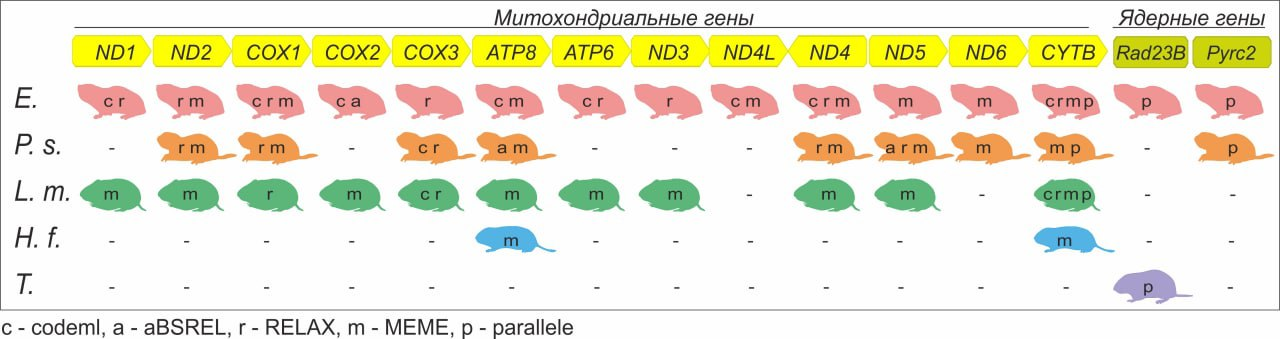
\includegraphics[width=\textwidth]{genes_mt_and_nucl}
	\end{center}
	\caption{Гены с достоверными изменениями уровня отбора для каждого из подземных видов. Буквы внутри каждого силуэта обозначают анализы, в которых был получен достоверный результат. E --- виды рода \textit{Ellobius}, P.s. --- \textit{P. schaposchnikowi}, L.m. --- \textit{L. mandarinus}, H.f. -- \textit{H. fertilis}, T. — виды рода \textit{Terricola}.} \label{Convergent_arv}
\end{figure}

 Самыми стрессовыми факторами, с которыми сталкиваются подземные грызуны, являются гипоксические / гиперкапнические условия и перегрев в закрытой системе нор (\cite{Lacey2000}). Хотя и слепушонки, и \textit{P.schaposchnikowi} являются высокоспециализированными подземными грызунами, они занимают разные среды обитания, и характеристики их нор, а также методы добычи пищи весьма различны. Типичные места обитания \textit{Ellobius} --- засушливые или полузасушливые ландшафты, такие как степи, пустыни и луга. Эти грызуны населяют различные типы почв, в том числе плотные почвы глинистых пустынь, и создают довольно устойчивые системы узких туннелей для кормления под землей (\cite{Ognev1950}; \cite{Gromov1977}; \cite{Shubin1978}). Таким образом, слепушонки должны справляться с проблемами, с которыми сталкиваются другие действительно подземные млекопитающие (\cite{Lacey2000}). Последнее, в свою очередь, может привести к наблюдаемым нами изменениям в белок-кодирующих генах. Напротив, \textit{P.schaposchnikowi} встречается на кавказских субальпийских высокотравных лугах на высоте 1500-2500 м (\cite{Vereshchagin1959}; \cite{Vorontsov1966}; \cite{Krystufek2005}). Его норы вырыты в рыхлой влажной почве, заполненной камнями, что должно увеличить диффузию газа. Важно отметить, что поверхностные кормовые туннели этих полевок необычны тем, что они кажутся слишком большими и почти вдвое шире, чем можно было бы ожидать от грызунов такого размера (\cite{Vorontsov1966}; личные наблюдения А.В. Сморкачевой). Это дополнительное пространство может предотвратить перегрев, гипоксию и гиперкапнию. Кроме того, \textit{P.schaposchnikowi} строго травояден, по крайней мере, летом. Во время кормления полевка высовывается из норы, подбирает растения и затаскивает их в нору для безопасного кормления (\cite{Gambaryan1957}; \cite{Zimina1977}; личные наблюдения А.В. Сморкачевой). Таким образом, даже будучи ограниченными в поисках пищи вблизи отверстий для нор, они на самом деле проводят много времени вне туннелей. Благодаря холодному климату, архитектуре нор и особенностям кормления, \textit{P.schaposchnikowi} может избежать некоторых физиологических проблем, с которыми приходится сталкиваться большинству подземных видов.

У \textit{L. mandarinus}, несмотря на обнаруженные ранее изменения в циркадных ритмах и адатпации к гипоксии (\cite{Sun2018}; \cite{Dong2020}), мы наблюдаем не такие сильные изменения в изученных нами генах: всего три гена с изменением уровня отбора --- \textit{COX1}, \textit{COX3} и \textit{CYTB}. Тем не менее, мы обнаружили существенные различия у \textit{Lasiopodomys mandarinus} и \textit{Terricola}, несмотря на схожий эволюционный возраст этих таксонов. Это различие также может отражать неравные уровни энергетического и гипоксического стресса, возникающие из-за специфических характеристик стратегии поиска пищи и архитектуры норы. \textit{Lasiopodomys mandarinus} питаются либо под землей, либо зелеными частями растений в непосредственной близости от входа в нору. Кормовые ходы этого вида расположены на глубине 10-30 см (\cite{Smorkatcheva1990}; \cite{Hong2019}), а прямые измерения концентрации газов, температуры и влажности подтвердили, что животные в норе должны столкнуться с гипоксией и гиперкапнией. \textit{Terricola} населяют различные растительные сообщества от широколиственных лесов (\textit{T. subterraneus}) до альпийских лугов (\textit{T. daghestanicus}) (\cite{Aulagnier2018}). Подобно \textit{Ellobius}, \textit{Prometheomys} и \textit{L. mandarinus}, они используют сложную сеть подземных тоннелей и демонстрируют некоторые внешние черты, связанные с подземным образом жизни (\cite{Aulagnier2018}; \cite{Mironov2020}). Однако телосложение и повадки \textit{T. subterraneus} (Абрамсон и Сморкачева, неопубликовано), а также характеристики его туннельной системы отличают эту полевку от специализированных подземных грызунов. Пищевые пути этого вида располагаются в самом поверхностном слое почвы (в пределах 5--10 см) или даже непосредственно под опадом листьев (\cite{Mironov2020}). Туннели обеспечивают защиту полевок от неблагоприятных погодных условий и хищников, что объясняет тенденцию видов \textit{Terricola} к снижению скорости базовых метаболических процессов (\cite{Caroli2000}; \cite{Jemiolo1983}; \cite{Schropfer1977}), но их глубина, вероятно, слишком мала, чтобы существенно предотвратить диффузию газа, приводящую к гипоксическим / гиперкапническим условиям внутри. К сожалению, об экологии \textit{T. daghestanicus}, населяющего кавказские альпийские степи и луга, почти ничего не известно. Тот факт, что полевки этого вида, как сообщается, находят убежище среди скал (\cite{Krystufek2005}), предполагает, что они не так строго подземные. Наши результаты подтверждают этот факт, поэтому мы не обнаружили никаких изменений уровня отбора в митохондриальных генах этого вида. 

 Подземные полевочьи повторяют адаптационный путь других подземных грызунов, показывая схожие признаки (таблица \ref{convergent_all}). Так, во время многочисленных исследований представителей семейств Bathyergidae и  Spalacidae были обнаружены параллельные замены в абсолютно разных генах. Также во многих генах видно ослабление отбора и увеличение его уровня по сравнению с наземными. Этот эволюционный тренд подтверждается не только на подземных грызунах, но и на других подземных млекопитающих --  Talpidae и Chrysochloridae. Обнаруженные адаптации митохондриального генома (увеличение уровня отбора, наличие параллельных замен) совпадают с исследованиями на Octodontidae и Ctenomyidae. Таким образом, полученные нами результаты согласуются с гипотезой о том, что переход к подземному образу жизни стимулирует ослабление уровня отбора. Причем выраженность скорее связана с уровнем специализации вида, нежели с возрастом его появления.


%\begin{landscape}
%	
%	\begin{table}[]
%		\caption{Конвергентная эволюция у подземных Arvicolinae. MT -- митохондриальный геном, RNA -- транскриптом. NA -- анализ не проводился, нет -- признаки отсутствуют.}\label{convergent} \vspace{5mm}
%		
%		\begin{tabular}{|c|p{5cm}|p{3.5cm}|p{3.5cm}|p{3.5cm}|p{3.5cm}|p{3.5cm}|}
%			\hline
%			&  & \multicolumn{1}{c|}{\textit{Ellobius sp.}} & \multicolumn{1}{c|}{\textit{P. schaposchnikowi}} & \multicolumn{1}{c|}{\textit{Terricola}} & \multicolumn{1}{c|}{\textit{L. mandarinus}} & \multicolumn{1}{c|}{\textit{H. fertilis}} \\ \hline
%			\multirow{2}{*}{MT} & Гены под отбором & \textit{ATP}6,8,   \textit{COX}1-2, \textit{ND}1, 4, 4L & \textit{COX3} & нет & \textit{COX3}, \textit{CYTB} & нет \\ \cline{2-7}
%			& Параллельные   замены & \textit{CYTB}– 56, 338 & \textit{CYTB} – 56 & нет & \textit{CYTB} – 56, 338 & нет \\ \hline
%			\multirow{2}{*}{RNA} & Гены под отбором & нет & нет & нет & нет & NA \\ \cline{2-7}
%			& Параллельные   замены &  \textit{Rad23b}, \textit{Pycr2} & \textit{Pycr2}& \textit{Rad23b} & нет & NA \\ \hline
%		\end{tabular}
%	\end{table}
%	
%\end{landscape}

\begin{landscape}

\begin{table}[]
	\caption{Конвергентная эволюция у подземных млекопитающих. MT -- митохондриальный геном.}\label{convergent_all} \vspace{5mm}
	
	\begin{tabular}{|p{3cm}|p{3cm}|p{2.8cm}|p{2.7cm}|p{3.4cm}|p{2.7cm}|p{3.3cm}|p{2.8cm}|}
		\hline
		\multicolumn{1}{|c|}{} & \textbf{Arvicolinae (\textit{Ellobius, Prometheomys, Lasiopodomys})} & \textbf{Octodontidae (\textit{Spalacopus})} & \textbf{Ctenomyidae (\textit{Ctenomys})} & \textbf{Bathyergidae (\textit{Heterocephalus, Fukomys, Cryptomys})} & \textbf{Talpidae (\textit{Condylura})} & \textbf{Chrysochloridae (\textit{Amblysomus, Chrysoschoris})} & \textbf{Spalacidae (\textit{Spalax})} \\ \hline
		Ослабление очищающего отбора (МТ) & увеличение уровня & увеличение уровня & увеличение уровня & нет данных & нет данных & нет данных & нет данных \\ \hline
		Ослабление очищающего отбора (ядерные гены) & как у наземных & нет данных & нет данных & увеличение уровня & увеличение уровня & увеличение уровня & увеличение уровня \\ \hline
		Параллельные замены & \textit{Rad23b, Pycr2, CYTB} & нет данных & нет данных & \textit{ARG1, A2M, ABCC3...} & \textit{A2M, ABCC3, C3...} & \textit{A2M, ABCC3, C3...} & \textit{ARG1, A2M...} \\ \hline
	\end{tabular}
\end{table}

\end{landscape}